\newpage
\section{Research Plan}

This work proposes a novel security framework for end-to-end generalist robots to address the inherent challenges of ensuring robustness, security, and trustworthiness in general-purpose robots across various physical embodiments. 
End-to-end generalist robot models leverage high-capacity models (\eg ViTs, LLMs, VLMs, and VLAs) pre-trained using Internet-scale data and training pipelines that use specific and/or \xot robotics datasets. 
The core concept relies on the systematic evaluation and discovery of potential vulnerabilities in all layers of the robotic learning stack. This plan describes the research tasks in this project.


\subsection{T0: Building Comprehensive Repository for End-to-end Robotic Models and Data}
% ~\vspace{-3ex}
\begin{wraptable}{r}{0.5\textwidth}\vspace{-3.5ex}
% \begin{table}
\centering
\caption{{Datasets augmenting OXE~\cite{9} for robots (\textbf{R}), \textbf{F}ranka, \textbf{G}oogle Robot, \textbf{S}pot, \textbf{H}ello Stretch, \textbf{U}R5, Hu\textbf{M}an}, and \textbf{X}arm7, with control frequency (\textbf{Hz}) and \textbf{\#} of episodes.}
\label{tab:multi_dataset}\vspace{-2ex}
\resizebox{0.99\linewidth}{!}{%
\begin{tabular}{lcclc}
\toprule
Dataset                     & \textbf{R}         &\textbf{ \#} & {Action Space}                           & \textbf{Hz}           \\
\midrule
 Franka  \cite{rosete2022tacorl,mees23hulc2}        & F       & 3242        & EEF Position                           & 15                            \\
Maniskill     \cite{gu2023maniskill2}               & F        & 30000       & EEF Position                           & 20                                               \\
Robocook   \cite{shi2023robocook}        & F       & 2460        & EEF Position                           & 5                                                \\
CMU Pick-Insert \cite{saxena2023multiresolution} & F        & 520         & EEF Position                           & 20                                      \\
RoboVQA  \cite{9}                       & G  & 61153       & EEF Position                           & 10                                                     \\
DROID \cite{khazatsky2024droid}                         & F        & 92233       & EEF Position                           & 15                                          \\
ConqHose  \cite{ConqHoseManipData}                     & S          & 139         & EEF velocity                           & 30                                          \\
DobbE   \cite{shafiullah2023dobbe}                     & H & 5208        & EEF Position                           & 3.75                                        \\
FMB \cite{luo2024fmb}                           & F        & 1804        & EEF velocity                           & 10                                                  \\
IO-AI Office \cite{9}    & M        & 3847        & EEF Position                           & 30                                                       \\
RoboSet\cite{bharadhwaj2023roboagent}                     & F        & 18250       & Joint position                         & 5                                        \\
VIMA \cite{jiang2023vima}                        & U          & 660103      & Primitive skills                       & NA                                               \\
SPOC \cite{spoc2023}                       & H & 233000      & Joint position                         & 10                                                     \\
Ours & X & 10000 & EEF/joint Position & 5-50 \\
\bottomrule
\end{tabular}}\vspace{-2ex}
\end{wraptable}
To conduct research tasks toward assessing and enhancing robustness, trustworthiness, and performance of robotic foundation models, we will build/train/evaluate various models using state-of-the-art techniques and \xot robotic data.\\
\BfPara{Robotics Data Mixture} We consider a multimodal robotics data mixture of
six robot embodiments (Franka, Google Robot, Spot, Hello Stretch, UR5, and Xarm7; \textit{fewer than the 22 embodiments in the OXE~\cite{9} dataset, for multimodality and practical reasons}) in addition to human demonstration data (see \autoref{tab:multi_dataset}). The mixture draws from 15 dataset sources: 14 robotics datasets (\autoref{tab:multi_dataset}, including our own for Xarm7) and the Open X-Embodiment (OXE)~\cite{9} repository, which itself aggregates 60 further robotic datasets.
% Freiburg Franka Play~\cite{rosete2022tacorl,mees23hulc2},
% Maniskill~\cite{gu2023maniskill2},
% Stanford Robocook~\cite{shi2023robocook},
% CMU Franka Pick-Insert Data~\cite{saxena2023multiresolution},
% RoboVQA~\cite{9},
% DROID~\cite{khazatsky2024droid},
% ConqHose~\cite{ConqHoseManipData},
% DobbE~\cite{shafiullah2023dobbe},
% FMB~\cite{luo2024fmb},
% IO-AI Office PicknPlace~\cite{9},
% RoboSet~\cite{bharadhwaj2023roboagent},
% VIMA~\cite{jiang2023vima},
% SPOC~\cite{spoc2023},
% and complemented by data taken from 
% RT-1~\cite{rt-1}, 
% QT-Opt~\cite{kalashnikov2018qt}, 
% Bridge~\cite{walke2023bridgedata}, 
% Jaco Play~\cite{dass2023jacoplay}, 
% Cable Routing~\cite{luo2023multistage}, 
% NYU VINN~\cite{pari2021surprising}, 
% Berkeley Autolab UR5~\cite{BerkeleyUR5Website}, 
% TOTO~\cite{zhou2023train} and 
% Language Table~\cite{lynch2023interactive} datasets.
% These datasets contain multiple modalities that are used to train RT-1-X and RT-2-X~\cite{9}.
% RT-1-X is trained on only the robotic data defined above, while RT-2-X is trained by co-fine-tuning (similarly to the original RT-2~\cite{rt-2}), with an approximately one-to-one split of the original VLM data and the robotics data mixture.
% Note, this data mixture includes data for 9 embodiments which is fewer than the entire OXE dataset (\ie 22) -- the practical reason for this difference is that we have continued to extend the dataset over time, and at the time of the experiments, the dataset above represented all of the data. In the future, 
We plan to continue extending our dataset (\ie added tasks and episodes) as we continue in our research and this project. 
% Other datasets, \ie for other embodiments, can and will be added to our repository when available to the research community.



\BfPara{End-to-end Models}
We identify two main families of end-to-end robotic foundation models: policy prediction models (\eg VLAs) and goal-conditioned models (\eg RoboCat~\cite{bousmalis2023robocat}). VLAs predict the next action based on the current state and instruction, while the second family, goal-conditioned models, predicts the next state based on the current state and goal. VLAs are gaining more traction due to their ability to leverage large pre-trained models and fine-tune them for specific tasks/embodiments (see~\autoref{fig:vla-timeline}).
{In the following, we describe the main models that we will use in this project. We will continue to expand the list of models as new models are released and/or become available for research use.}

\noindent\textbf{\cib{1} RT-1~\cite{rt-1} and RT-1-X~\cite{9}} RT-1 is a 35M parameter network built on a transformer architecture~\cite{vaswani2017attention} and designed for robotic control. %, as {shown} in~\autoref{fig:rtx}. 
It takes in a history of images (\eg 5 to 15 images) of resolution $300\times300$ along with the natural language instructions. 
Each image is processed through an ImageNet-pre-trained EfficientNet-B3~\cite{tan2019efficientnet} to output spatial feature maps of shape $9\times9\times512$ from the final convolutional layer.
The model was chosen primarily to balance accuracy, model size, and speed, keeping the local processing rate within 3Hz for the entire pipeline.
% \begin{wrapfigure}{r}{0.3\textwidth}{\vspace{-4.5ex}}
%   \centering
%   \includegraphics[width=0.29\textwidth]{figures/rt-1.pdf}\vspace{-2ex}
%       \caption{
%     \small RT-1-(X) and RT-2-(X) variations for {\xo}-embodied robotics.
%     }\vspace{-2ex}
%   \label{fig:rtx}
% \end{wrapfigure}
The natural language instruction is transformed into a USE~\cite{cer2018universal} embedding. 
The visual and language representations are then interwoven via FiLM~\cite{perez2017film} layers, producing 81 vision-language tokens. 
These tokens are fed into a decoder-only transformer that outputs the tokenized actions.
To tokenize actions, each action dimension in RT-1 is discretized into $256$~bins. 
The action dimensions we consider include seven variables for the arm movement ($x$, $y$, $z$, roll, pitch, yaw, opening of the gripper), three variables for base movement ($x$, $y$, yaw), and a discrete variable to switch between three modes: controlling arm, base or terminating the episode.
For example, an action
``$\Delta \textit{pos}_x\text{=}0.1 \enspace \Delta \textit{pos}_y\text{=}-0.2 \enspace \Delta \textit{pos}_z\text{=}0 \enspace \Delta \textit{rot}_x\text{=}10^{\circ} \enspace \Delta \textit{rot}_y\text{=}25^{\circ} \enspace \Delta \textit{rot}_z\text{=}-7^{\circ}
$'' for the arm could be represented as ``\textit{132 114 128 5 25 156}''.
For each variable, the target action/value is mapped to a value from the 256 bins, where the bins are uniformly distributed within the bounds of each variable. The {loss}
used for RT-1 training is a standard categorical cross-entropy entropy and causal masking that was utilized in prior transformer-based controllers~\cite{reed2022generalist,lee2022multi}. 
We use the same implementation/design choices for RT-1 model as reported by the original work. Other variations of RT-1, \eg different base/backbone models and operation modes (\ie local or cloud-based inference), will be implemented as RT-1-X designs.


\noindent\textbf{\cib{2} RT-2~\cite{rt-2} and RT-2-X~\cite{9}} RT-2 is a large (12--55B parameters) VLA model trained on Internet-scale vision and language data, along with robotic control data. 
RT-2 casts the tokenized actions as text tokens.
As such, any pre-trained VLM (\eg Pali-X~\cite{chen2023palix}, Flamingo~\cite{alayrac2022flamingo}, {P}a{LM}-E~\cite{driess2023palme}) can be fine-tuned for robotic control, thus leveraging the backbone of VLMs and transferring some of their generalization properties.
Action encoding and discretization are performed as in \cite{rt-1} for the RT-1 model. 
To fine-tune a VLM into a VLA model, tokens should be associated with the discrete action bins (\ie reserving 256 tokens to serve as action tokens). 
In order to define a target for VLM fine-tuning, the action vector is represented by a single string that simply concatenates action tokens for each dimension with a space character:
For example, a possible instantiation of the target,
``$\textit{terminate} \enspace \Delta \text{pos}_x \enspace \Delta \textit{pos}_y \enspace \Delta \textit{pos}_z \enspace \Delta \textit{rot}_x \enspace \Delta \textit{rot}_y \enspace \Delta \textit{rot}_z \enspace \textit{gripper\_extension}
$'',
could be: ``\textit{1 128 91 241 5 101 127}''.
To ensure that RT-2 outputs valid action tokens during decoding, the output vocabulary is
constrained to only sampling valid action tokens when the model is prompted with a robot-action task.
We note that the model, \ie the orginal VLM, can still output the full range of language tokens on standard vision-language tasks.
Our implementation focuses on the RT-2-PaLI-X variants~\cite{chen2023palix} built on the backbone of ViT~\cite{dosovitskiy2021image} visual model and UL2~\cite{tay2023ul2} language model, and pre-trained on WebLI~\cite{chen2023palix} dataset. %Variations of RT-2 will be implemented as RT-2-X designs for \xod training.

\begin{wraptable}{r}{0.5\textwidth}
\centering
\vspace{-2ex}
\caption{{\small Possible VLMs (and variations) for RT-2-X.}}
\label{tab:VLMs}
\vspace{-2ex}
\scalebox{0.73}{
\begin{tabular}{llll}
\toprule
Model & LLM & Adapter & Vision \\ \midrule
Flamingo~\cite{alayrac2022flamingo} & Chinchilla & Attention & NFNet-F6 \\
OpenFlamingo~\cite{awadalla2023openflamingo} & MPT & Attention & CLIP ViT-L \\
SPHINX-X~\cite{gao2024sphinx} & Mixtral & Linear & Mixture \\
Qwen-VL~\cite{bai2023qwen} & Qwen & Q-Former & ViT-bigG \\
BLIP-2~\cite{li2023blip} & Flan-T5/OPT & Q-Former & EVA ViT-g \\
InstructBLIP~\cite{dai2024instructblip} & Vicuna & Q-Former & EVA ViT-g \\
BLIVA~\cite{hu2024bliva} & Vicuna & Q-Former & EVA ViT-g \\
MiniGPT-4~\cite{zhu2023minigpt} & Vicuna & Linear & EVA ViT-g \\
MiniGPT-v2~\cite{chen2023minigpt} & LLaMA-2 & Linear & EVA ViT-g \\
LLaVA~\cite{liu2024visual} & Vicuna & Linear & CLIP ViT-L \\
LLaVA-1.5~\cite{liu2024improved} & Vicuna-v1.5 & MLP & CLIP ViT-L \\
LLaMA Adapter-V2~\cite{gao2023llama} & LLaMA & Linear & CLIP ViT-L \\
PandaGPT~\cite{su2023pandagpt} & Vicuna & Linear & ImageBind \\
\bottomrule
\end{tabular}}\vspace{-2ex}
\end{wraptable}
We will explore the adoption of other existing VLMs in the RT-2-X implementation for \xod training. 
\autoref{tab:VLMs} lists common open-source VLMs along with their respective components.
Typically, a VLM is composed of three key elements: a visual encoder (\ie vision model), an adapter, and an LLM backbone. 
The visual encoder extracts visual features from the input images, facilitating subsequent LLM reasoning and understanding of visual semantics. 
The most used visual encoders are pre-trained ViT models, with popular choices including the ViT-L model from CLIP \cite{radford2021learning} and the ViT-g from EVA-CLIP \cite{fang2023eva}. 
In addition to ViT-based models, other approaches employ ImageBind \cite{girdhar2023imagebind} and NFNet-F6 \cite{brock2021high}, among others, as visual encoders.
The adapter module connects the visual and textual input modalities. 
VLMs use various adapters, from basic architectures such as linear layers and MLPs to advanced ones such as Q-Former \cite{li2023blip} and cross-attention \cite{vaswani2017attention}.
For the LLM component, the LLaMA family is commonly preferred as the LLM backbone, primarily due to its open source status and the range of versions available to suit different requirements/capacities, such as LLaMA \cite{touvron2023llama}, LLaMA-2 \cite{touvron2023llama2}, Vicuna, and Vicuna-v1.5 \cite{chiang2023vicuna}. 
Other LLM backbones include Flan-T5 \cite{chung2024scaling}, MPT \cite{mosaicml2023introducing}, Chinchilla \cite{hoffmann2022training}, OPT \cite{zhang2022opt}, Mixtral \cite{jiang2024mixtral}, and Qwen \cite{bai2023aqwen}. 
We plan to explore variations of VLMs in building RT-2-X and evaluate the impact of architecture design on the development of robotic models. %Similarly, multiple vision models with the RT-1-X design will be evaluated.

% \noindent\textbf{\cib{3} } Variants of RT-1 and RT-2 with different base/backbone models will be implemented to assess the impact of design choices on performance and robustness of models. In addition, we will evaluate the impact of incorporation of various datasets, including \xot datasets, on the generalization, performance, and robustness of models.
% We note that other implementations of generalist robotic models, \eg ~{MOO}~\cite{stone2023open} will be included in our evaluation. {MOO}~\cite{stone2023open} employs a VLM to generate an additional image channel for a semantic map, which is subsequently fed into an RT-1 backbone.

\noindent\textbf{{\cib{3}} OpenVLA and [X]-VLA Variants} 
OpenVLA~\cite{kim2024openvla} (7B parameters)
is an open-source alternative to RT-2~\cite{rt-2}. % that is built on the open-source VLMs.
OpenVLA, as other VLAs, follows the same design principles that include training/fine-tuning open-source VLMs which consist of three components: vision tokenizer/encoder/adapter, LLM backbone, and action decoder/tokenizer. 
OpenVLA uses Prismatic VLM (7B-parameter) and is trained on 970k real-world robot demonstrations outperforming larger models like RT-2 ($\sim$55B). The Prismatic VLM uses dual vision encoders (DINOv2 \cite{oquab2023dinov2} and SigLIP \cite{zhai2023sigmoid}) and a LLaMA-2 language model \cite{touvron2023llama}.
Variants of OpenVLA, \eg  ReVLA~\cite{dey2024revla}, Edge-VLA~\cite{budzianowski20edgevla}, PointVLA~\cite{li2025pointvla}, and CoVLA~\cite{arai2025covla} (see \autoref{fig:vla-timeline}), have been proposed to improve the original design in terms of performance, efficiency, reasoning, and/or specialty.
Similar to RT-2-X, we will adopt various open-source VLMs/components (in \autoref{tab:VLMs}) to build/train [X]-VLA variants.


\noindent\textbf{\cib{4} RoboCat~\cite{bousmalis2023robocat}} RoboCat follows a different approach by conditioning the model on visual goal. The architecture is VQ-GAN encoder which is based on the Gato architecture~\cite{esser2021taming} that processes the image (with $128\times128$ resolution) as $8\times8$ tokens and outputs encoded vectors. These vectors are then discretized via a nearest-neighbor lookup in a codebook of embeddings.
The VQ-GAN encoder is a ResNet~\cite{resnet} with 2 groups of 2 blocks, followed by 3 attention layers. 
The decoder has 3 attention layers followed by a ResNet with 2 groups of 3 blocks. %The vector quantiser~\citep{van2017neural} uses 64 embeddings of dimension 128. 
For tokenization of observations and actions, RoboCat follows a similar approach as~\cite{reed2022generalist}.
The loss is weighted as ($0.25\times\text{discretization\_loss} + \text{l2\_reconstruction\_loss} + 0.1\times\text{log\_laplace\_loss}$) to predict future tokens. The output is the image tokens at time step $k = 5$, as one step can look very similar.

\noindent\textbf{\cib{5} Octo~\cite{team2024octo}} Octo is a (27-93M parameters) transformer-based VLA pre-trained on the OXE~\cite{9} dataset. Unlike RT-X and RoboCat, it can be fine-tuned to new observations and action spaces. This flexibility allows Octo to adapt to various robotic embodiments, a trend that is becoming increasingly important/adopted in robotics.
Octo architecture consists of three key parts: \textit{input tokenizers} that transform language instructions and observations into tokens, a \textit{transformer backbone} that receives the tokens and generates embeddings, and \textit{readout heads} that produce the desired outputs, \ie actions. Input tokenizers include modality-specific tokenizers, \ie a language (task) tokenizer (\eg T5) and a vision tokenizer (\eg ViT-based or CNN-based). Unavailable modalities are masked (\eg no language instructions are provided), and learnable position embeddings are added to the input tokens before feeding them into the transformer backbone.  Octo also uses a \textit{readout token} analogous to the $\text{[CLS]}$ token in BERT/LLMs.
The transformer backbone processes the input tokens through block-wise masked attention patterns (\ie see to tokens from the same or earlier time steps), which are then passed to the readout heads. The readout ``\textit{action}'' head predicts a ``\textit{chunk}'' of several consecutive actions.
Action heads can be added/replaced/fine-tuned during downstream fine-tuning (\eg adoption of new embodiments).


\noindent\textbf{\cib{6} ACT~\cite{zhao2023learningFB}} ACT is a VLA model that uses ResNet~\cite{resnet} as the vision encoder and transformer-based
conditional variational autoencoder (CVAE)~\cite{sohn2015learning} that generates a sequence of actions. The original ACT 
\begin{wrapfigure}{r}{0.45\textwidth}{\vspace{-2ex}}
  \centering
\begin{minipage}{0.45\textwidth}
      \centering
        \begin{minipage}{\linewidth}
          \centering
          \begin{minipage}{0.33\linewidth}
            \centering
            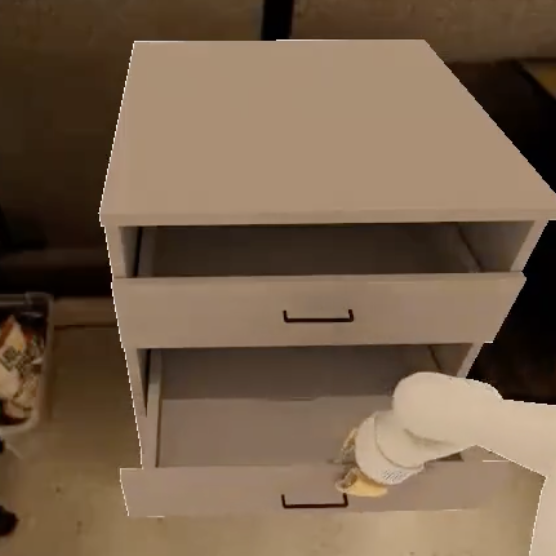
\includegraphics[width=\textwidth]{figures/examples/1.png}
          \end{minipage}%
          \begin{minipage}{0.33\linewidth}
            \centering
            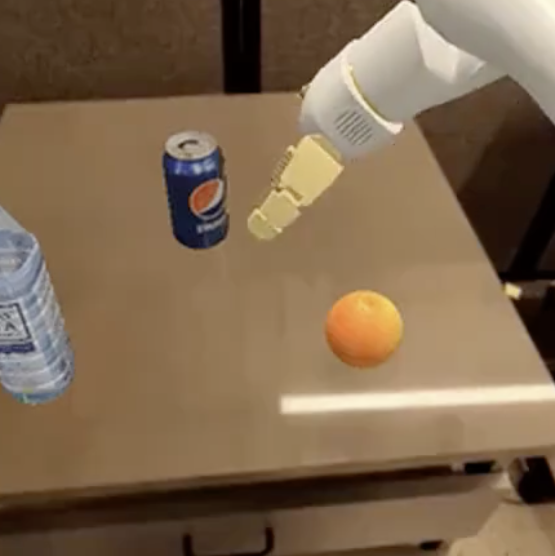
\includegraphics[width=\textwidth]{figures/examples/2.png}
          \end{minipage}%
          \begin{minipage}{0.33\linewidth}
            \centering
            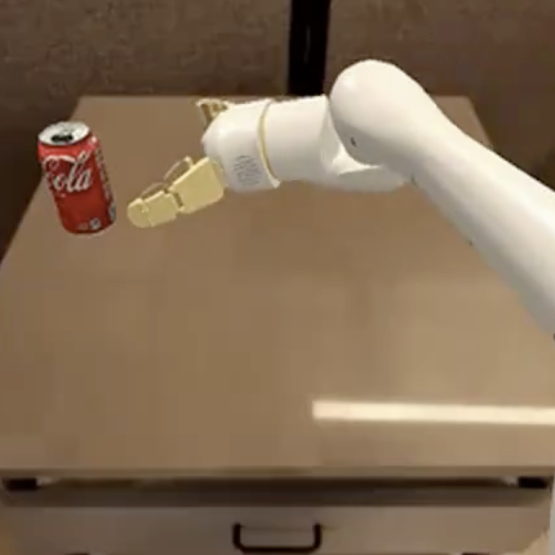
\includegraphics[width=\textwidth]{figures/examples/3.png}
          \end{minipage}
        \end{minipage}\vspace{-1.5ex}
        \begin{minipage}{\linewidth}
          \centering
          \begin{minipage}{0.33\linewidth}
            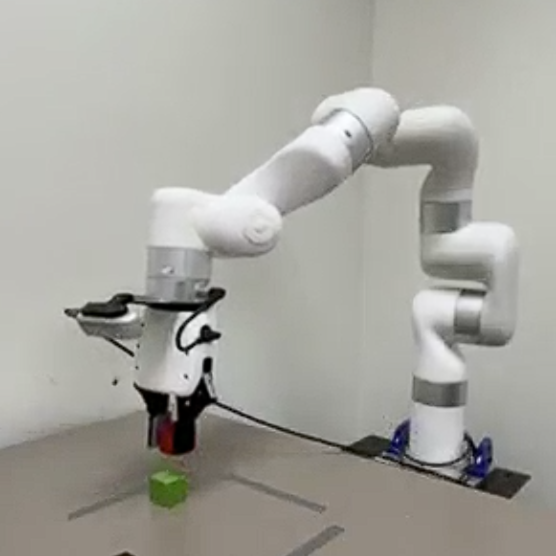
\includegraphics[width=\textwidth]{figures/examples/4.png}
          \end{minipage}%
          \begin{minipage}{0.33\linewidth}
              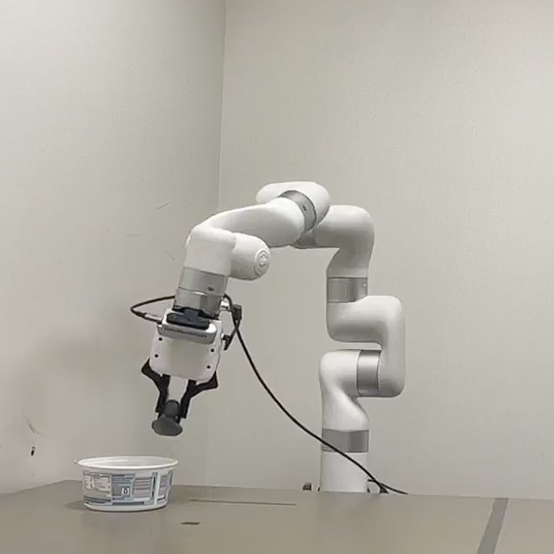
\includegraphics[width=\textwidth]{figures/examples/5.png}  
            \end{minipage}%
          \begin{minipage}{0.33\linewidth}
            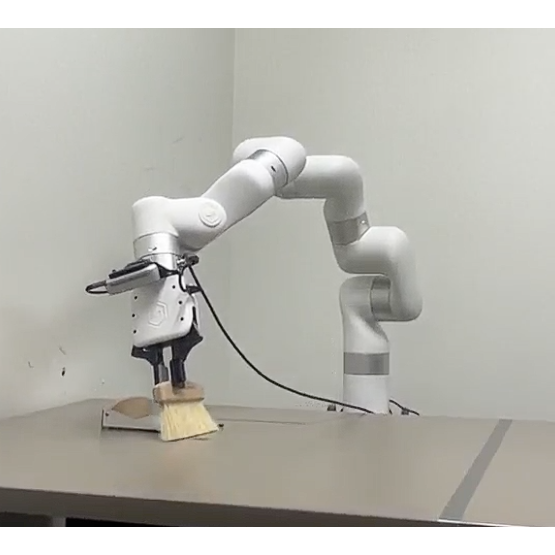
\includegraphics[width=\textwidth,trim={10pt 0 50pt 0},clip]{figures/examples/6.png}
          \end{minipage}\vspace{-2.5ex}
          \caption{\textbf{(Top)} Simulation tasks from Simpler~\cite{li24simpler}: {Close drawer}, {Move closer}, and {Pick Coke Can}. \textbf{(Bottom)} 
          Xarm7: {Stack Cubes}, {Duck in Bowl}, and {Sweep}.}
          \label{fig:xarm7}
        \end{minipage}
    \end{minipage}%
  \hfill
    \begin{minipage}{0.45\textwidth}
      \centering
      \begin{minipage}{0.45\linewidth}
        \centering
        \includegraphics[width=\textwidth]{figures/results/sim_res.pdf}
      \end{minipage}
      \hfill
      \begin{minipage}{0.49\linewidth}
        \centering
        \includegraphics[width=\textwidth]{figures/results/real_res.pdf}
      \end{minipage}
      \vspace{-2.5ex}
      \caption{Performance of models on simulated (left) and real (right) robotic tasks.}
      \label{fig:res}
    \end{minipage}\vspace{-2ex}
\end{wrapfigure}
was designed to process visual data and joint positions without additional language instructions. 
Similar to Octo~\cite{team2024octo}, ACT processes the images (multiple views if available, \eg original ACT uses 4 camera views) through a ResNet model, adds positional embeddings, and feeds them into a transformer-based CVAE-encoder (along with joint positions) to generate a sequence of actions (projected using MLP to chunks of absolute joint positions) through the CVAE-decoder.
For example, for Bimanual robots, the observation includes 4 RGB images (4 cameras), each at $480\times640$ resolution, and joint positions for two robot arms (7+7=14 positions in total).
The ResNet processes each image ($480\times640\times3$) and outputs feature maps of 4 images $\times$ $15\times20\times512$.
These feature maps are flattened ($1200\times512$), added to positional embeddings, and fed into the transformer encoder with additional joint position information.
The transformer decoder processes the encoder output through cross-attention to generate a sequence of actions ($k \times 512$ where $k$ is the number of action chunks). To generate the final actions, the output is down-projected with an MLP to $k \times 14$ dimensions, corresponding to the target joint positions for the next $k$ steps.
Our implementation of ACT will follow the original design choices, but changes are adopted to accommodate data from other embodiments, which can change the number of views and action dimensions, \eg the Xarm7 robot has 1 camera view (additional views can be added) and 7 action dimensions (7 degree-of-freedom positions).






\BfPara{Preliminary Experiments: Robotic Models} 
We have conducted preliminary experiments to evaluate the performance of robotic models, \ie RT-1, RT-2, Octo, and ACT on simulated and real robotic tasks. 
For simulation, we used Simpler~\cite{li24simpler} benchmark for three tasks: \emph{Close the drawer}, \emph{Move closer}, and \emph{Pick the Coke Can} using Google robot embodiment, while for real experiments, we used Xarm7 robot for three tasks: \emph{Stack Cubes}, \emph{Duck in Bowl}, and \emph{Sweep} (see~\autoref{fig:xarm7}).
For the simulation tasks, models were fine-tuned (using single third-person view and language-conditioned control) using 50 episodes per task. Language instructions are not used for ACT. Five training runs were performed per model, where each run was trained for 20,000 iterations with a batch size of 512 and a learning rate of 1e-5 using AdamW optimizer. The evaluation was performed on 25 episodes per task over five runs with different random seeds.
Similar training and evaluation settings were used for the real robotic tasks, but with visual observations only and no language instructions to avoid any changes on the ACT model architecture. 
Task success is measured using a two-point scoring system. For \emph{Stack Cubes} (stacking two cubes) and \emph{Duck in a bowl} (placing duck in bowl), points are awarded for successful pick (1 point) and place (1 point) operations. For \emph{Sweep}, points are given for finding (1 point) and sweeping objects into the bin (1 point). The success rate is calculated as the average scores divided by the total points in all evaluation episodes.
The preliminary results are shown in~\autoref{fig:res}.

% \BfPara{Adoption and Constraints}
% At inference time, each model is required to run at the rate required for the robot (3-10~Hz). 
% While relatively small models, \eg ACT, Octo, RT-1 can run locally on some robots with such inference rate, larger models, \eg OpenVLA and RT-2 (7B+ parameters), are hosted on a cloud service and queried over the network. This can introduce latency and network reliability issues, which are critical for real-time robotic applications.
% Even when designing/training such models to generate chunks of actions at once, which can be executed over several time steps,
% robotic models require strict real-time performance for smooth operation. % unlike general LLM/VLMs which often operate without stringent timing constraints.
% This adds complexity to robotic models, \ie managing latency, network reliability, and data communication security aspects that are less critical in typical LLM/VLM applications.
% In terms of adversarial attacks, attacking a robot's availability through prompt injection or jailbreak attacks (\eg running prompts that take more than 15Hz) can have far more serious consequences than similar attacks on other LLM/VLM applications.
% Compromised availability (and/or functionality) of a robot from an attack can cause physical harm, property damage, or operational disruptions.
% The real-time and/or (network dependence) of these models adds vulnerabilities that can be exploited to disrupt availability, making it imperative to prioritize security and resilience against such attacks.




\subsection{T1: Vulnerability Analysis in Foundation Generalist Robots}

This task aims to secure emerging robotic foundation models, where security and robustness are crucial.
Vulnerabilities in AI models have been the focus of many studies recently, showing how small adversarial manipulations to the model's input can significantly impact their performance.
Adversarial machine learning has emerged as an active field of research that addresses various threats to AI systems.
Based on the NIST Trustworthy and Responsible AI report~\cite{NIST_AI_100_2e2023}, the taxonomy of the most studied and effective attacks includes \emph{evasion}, \emph{poisoning}, and \emph{privacy} attacks for predictive AI systems with the addition of \emph{abuse} attacks for generative AI systems.
Since end-to-end robotic models fall into the generative AI category, this task addresses all categories of attacks, including evasion, poisoning, privacy, and abuse attacks.
% Given the high-dimensional and multimodal nature of the search space for attacks aginst robotic models, simply introducing random noise to inputs might fail to identify subtle vulnerabilities of the robotic model.
% Moreover, robotic models/policies are generally designed to be resilient against such noise~\cite{miki2022scirob}, making such adversarial attacks ineffective using straightforward methods.







\BfPara{Challenges in Attacking Robotic Models} 
Attacking robotic models
presents unique challenges due to their complex architectures, the multimodal nature of their input, restrictions on the output/action space, and the evolving landscape of security measures. 
Understanding these challenges is crucial for developing effective attack strategies that help
uncover vulnerabilities and improve the robustness of these models. 
Main challenges include the following:
{\cib{1}} \textbf{{Multimodal Complexity}}: Generalist robotic models process/integrate data from multiple modalities, such as sensory/positions data, images, and text, to predict action sequences. We believe that the efforts to build robotic foundation models will continue to grow and other modalities will be incorporated.
    Creating effective attacks requires understanding and manipulating the intricate relationships and interactions among these modalities \cite{radford2021learning}. 
    Consequently, creating adversarial examples that can deceive both the visual and language components is more challenging than focusing on one. %, such as attacks on vision models~\cite{abdukhamidov2023hardening,abdukhamidov2024singleadv} and LLM~\cite{chowdhury2024breaking}, or unimodal attacks VLM \cite{fan2024unbridled}.
\\{\cib{2}} \textbf{{Model Scale and Complexity}}: Current end-to-end robotic models involve large architectures containing millions to billions of parameters, making them highly complex and computationally expensive to attack.
    Adapting traditional adversarial attacks from downstream tasks to successfully impact such large models necessitates significant computational resources and sophisticated optimization methods.
\\{\cib{3}} \textbf{{Attack Practicality and Transferability}}: 
    Adversarial scenarios against robotics should be practical, \ie scenarios in which robots are likely to face operational tasks. 
Therefore, attacks must be systematic and guided by practical experience in field robotics to ensure the plausibility and reflection of real-world scenarios. 
    Moreover, attack methods against similar LLMs/VLMs use white-, gray-, and black-box settings relying on prior knowledge of (exact or similar) models, training data, restrictions/constraints of the system or training a surrogate models. However, robotic applications and commercial vendors often do not share model details \cite{cheng2018query}. In practice, attackers can only query the model and observe the behavior of the robot/output of the model. Developing attacks that exploit multiple vulnerabilities \cite{biggio2018wild} or adapt to various threat vectors is necessary and requires versatile strategies.
    Moreover, an effective attack should be undetectable/imperceptible by human/robot observer, which requires preserving the semantic traits of the benign sample. 
    This requires well-designed constraints to restrict the type and size of the perturbation. 
    Numerous studies have shown that some attacks inhibit high transferability, \ie attacks on a given model can succeed on other similar models. This phenomenon derived the transfer-based black-box attacks.
    Nevertheless, attacks designed for similar LLMs/VLMs models might not always work effectively on other models, even if they share similar architectures. 
    Ensuring adversarial examples are transferable \cite{liu2016delving} across models and tasks requires understanding model-specific vulnerabilities and generalizable attack methods.





        % Highly improbable conditions, like disturbances significantly beyond normal environmental challenges, do not contribute effectively to our understanding of a controller's nuanced vulnerabilities. 
    
    %\item  \textbf{Interpretable and Explainable Attacks}: For attacks to be truly effective, attackers need to understand the internal workings and decision-making processes \cite{doshi2017towards} of VLMs. However, the black-box nature of many VLMs, coupled with their complexity, makes it difficult to interpret how and why an attack succeeds or fails.
    % \item  \textbf{Robustness to Defenses}: Many VLMs incorporate dynamic defense mechanisms that can adapt to detected adversarial activities. These defenses may include real-time monitoring, anomaly detection, and adaptive retraining. Therefore, attack strategies need to continuously evolve to stay ahead of these adaptive defenses, which require substantial computational resources and sophisticated algorithms.






\BfPara{Attacking Robotic Foundation Models}
~{Let $\mathcal{M}$ represent a robotic foundation model, which takes a tuple of inputs, \eg $(\{\bm{x}\}, \{\bm{t}\}, \{\bm{s}\}, \dots)$ representing input modalities (\ie a set (at least one) of images \{$\bm{x}\} \in \mathcal{X}$, set of text instructions \{$\bm{t}\} \in \mathcal{T}$, set of sensory/position data $\{\bm{s}\}\in \mathcal{S}$, and other available information) and outputs a set of tokenized actions $\mathcal{M}(\{\bm{x}\}, \{\bm{t}\}, \{\bm{s}\}, \dots)=\{\bm{a}_{out}\}$.
Since robots could have multiple embodiments/tasks (and various action spaces), some inputs could become a placeholder/masked $\oslash$ or nonexistent modified to fit the model.}
%%{\vspace{-2ex}}
% Let $\mathcal{M}$ represent a robotic foundation model, which takes a tuple of inputs, \eg $(\{\bm{x}\}, \{\bm{t}\}, \{\bm{s}\}, \dots)$ representing input modalities (\ie a set (at least one) of images \{$\bm{x}\} \in \mathcal{X}$, set of text instructions \{$\bm{t}\} \in \mathcal{T}$, set of sensory/position data $\{\bm{s}\}\in \mathcal{S}$, and other available information) and outputs a set of tokenized actions $\mathcal{M}(\{\bm{x}\}, \{\bm{t}\}, \{\bm{s}\}, \dots)=\{\bm{a}_{out}\}$.
% Since robots could have multiple embodiments/tasks (and various action spaces), some inputs could become a placeholder/masked $\oslash$ or nonexistent modified to fit the model.
For example, RT-2 and OpenVLA models receive only images and textual instruction $\mathcal{M}(\{\bm{x}\}, \{\bm{t}\})=\bm{a}_{out}$, 
%RoboCat and RT-1 receive images and no text, $\mathcal{M}(\{\bm{x}\}, \oslash)=\bm{a}_{out}$, 
Octo receives images, text, and sensory data $\mathcal{M}(\{\bm{x}\}, \{\bm{t}\}, \{\bm{s}\})=\bm{a}_{out}$, and ACT receives only images and sensory data $\mathcal{M}(\{\bm{x}\}, \{\bm{s}\})=\bm{a}_{out}$.
If Octo is used for robots/datasets that do not provide text instructions, the model processes available inputs and mask unavailable ones $\mathcal{M}(\{\bm{x}\}, \oslash,\{\bm{s}\})=\bm{a}_{out}$.
The output $\{\bm{a}_{out}\}$ is one or chunks of actions, each is a sequence of tokens representing predicted actions.



The attack operation $\mathcal{P}(.)$ is defined as a perturbation function that alters the inputs (one or more 
\begin{wraptable}{r}{0.5\textwidth}
\centering \vspace{-2ex}
\caption{{\small Stages (Training and Inference), targets (Privacy, Integrity, Availability, and Abuse) and types ( White- (\dd), Gray- (\bb), and Black-box (\vv) ) of common Evasion, Poisoning, and Privacy attacks.}}\vspace{-3.5ex}
\label{table:attacks_models}
\small
\resizebox{0.98\linewidth}{!}{%
\begin{tblr}{
rowsep=0pt,
  column{3} = {c},
  column{4} = {c},
  column{5} = {c},
  column{6} = {c},
  column{7} = {c},
  column{8} = {c},
  column{9} = {c},
  cell{2}{1} = {r=7}{},
  cell{10}{1} = {r=10}{},
  cell{20}{1} = {r=6}{},
  hline{2,10,20,26} = {-}{},
}
                                                  &                                & \begin{sideways}Training\end{sideways} & \begin{sideways}Inference\end{sideways} & \begin{sideways}Privacy\end{sideways} & \begin{sideways}Integrity\end{sideways} & \begin{sideways}Availability\end{sideways} & \begin{sideways}Abuse\end{sideways} & \begin{sideways}Type\end{sideways} \\
\begin{sideways}Evasion      ~\end{sideways}      & Indirect Prompt Injection      & \ee                                       & \checkmark                                         & \checkmark                                       & \checkmark                                         & \checkmark                                            & \checkmark                                     & \vv                          \\
                                                  & Universal Adversarial Triggers & \ee                                       & \checkmark                                         & \ee                                      & \ee                                        & \ee                                           & \checkmark                                     & \vv                          \\
                                                  & Gradient-based Attacks         & \checkmark                                        & \checkmark                                         & \ee                                      & \ee                                        & \ee                                           & \ee                                    & \dd                          \\
                                                  & Prompt Injection               & \ee                                       & \checkmark                                         & \checkmark                                       & \checkmark                                         & \checkmark                                            & \checkmark                                     & \bb                           \\
                                                  & Refusal Suppression            & \ee                                       & \checkmark                                         & \ee                                      & \ee                                        & \ee                                           & \checkmark                                     & \bb                           \\
                                                  & Style Injection                & \ee                                       & \checkmark                                         & \ee                                      & \ee                                        & \ee                                           & \checkmark                                     & \bb                           \\
                                                  & Role-play Strategies           & \ee                                       & \checkmark                                         & \ee                                      & \ee                                        & \ee                                           & \checkmark                                     & \bb                           \\
                                                  & Jailbreak           & \ee                                       & \checkmark                                         & \ee                                      & \ee                                        & \ee                                           & \checkmark                                     & \bb                           \\
\begin{sideways}Poisoning         ~\end{sideways} & Data Poisoning                 & \checkmark                                        & \ee                                        & \ee                                      & \checkmark                                         & \checkmark                                            & \ee                                    & \dd                          \\
                                                  & Model Poisoning                & \checkmark                                        & \ee                                        & \ee                                      & \checkmark                                         & \checkmark                                            & \ee                                    & \dd                          \\
                                                  & Backdoor Poisoning             & \checkmark                                        & \checkmark                                         & \checkmark                                       & \ee                                        & \ee                                           & \checkmark                                     & \dd                          \\
                                                  & Label Flipping                 & \checkmark                                        & \ee                                        & \ee                                      & \checkmark                                         & \checkmark                                            & \ee                                    & \dd                          \\
                                                  & Clean-label Poisoning          & \checkmark                                        & \ee                                        & \ee                                      & \ee                                        & \ee                                           & \ee                                    & \dd                          \\
                                                  & Targeted Poisoning             & \checkmark                                        & \ee                                        & \ee                                      & \ee                                        & \ee                                           & \ee                                    & \dd                          \\
                                                  & Subpopulation Poisoning        & \checkmark                                        & \ee                                        & \ee                                      & \ee                                        & \ee                                           & \ee                                    & \dd                          \\
                                                  & Model Replacement              & \checkmark                                        & \ee                                        & \ee                                      & \ee                                        & \ee                                           & \ee                                    & \dd                          \\
                                                  & Model Boosting                 & \checkmark                                        & \ee                                        & \ee                                      & \ee                                        & \ee                                           & \ee                                    & \dd                          \\
                                                  & Functional Attacks             & \checkmark                                        & \ee                                        & \ee                                      & \ee                                        & \ee                                           & \ee                                    & \dd                          \\
\begin{sideways}Privacy\end{sideways}             & Data Reconstruction            & \ee                                       & \checkmark                                         & \checkmark                                       & \ee                                        & \ee                                           & \ee                                    & \vv                          \\
                                                  & Membership Inference           & \ee                                       & \checkmark                                         & \checkmark                                       & \ee                                        & \ee                                           & \ee                                    & \bb                           \\
                                                  & Model Extraction               & \ee                                       & \checkmark                                         & \checkmark                                       & \ee                                        & \ee                                           & \ee                                    & \vv                          \\
                                                  & Property Inference             & \ee                                       & \checkmark                                         & \checkmark                                       & \ee                                        & \ee                                           & \ee                                    & \bb                           \\
                                                  & Attribute Inference            & \ee                                       & \checkmark                                         & \checkmark                                       & \ee                                        & \ee                                           & \ee                                    & \bb                           \\
                                                  & Prompt and Context Stealing    & \ee                                       & \checkmark                                         & \checkmark                                       & \ee                                        & \ee                                           & \ee                                    & \vv                          
\end{tblr}
}{\vspace{-3ex}}
\end{wraptable}
modalities, such as images, text, and sensory data) to mislead the model into producing an incorrect/unintended output action.
% We denote attacks on robotic models as $\mathcal{P} (.)$, which can be applied to one or more input modalities, \eg images, text, and sensory data.
For example, $\mathcal{P}(\bm{x})$ attacks image inputs $\bm{x}$, $\mathcal{P}(\bm{t}_{in})$ attacks text inputs $\bm{t}_{in}$, and $\mathcal{P}(\bm{x}, \bm{t}_{in})$ attacks both images and instructions.
\ul{Adversarial specificity} can be either \textbf{targeted} or \textbf{untargeted} against security concepts Integrity, Confidentiality, and Availability.
For simplicity, we denote attack specificity as $\mathcal{P}(.) \xrightarrow{{}_{\textbf{T}}}  \bm{a}_{out}'$ for targeted and $\mathcal{P}(.) \xrightarrow{{}_{\textbf{U}}}  \bm{a}_{out}'$ for untargeted attacks.
The \ul{attacks goals} can be categorized into \textbf{evasion}, \textbf{poisoning}, and \textbf{privacy}, and can be \ul{launched} either in \textbf{training} or \textbf{inference} phases.
For example, $\mathcal{P}(\bm{x},\bm{t}_{in}) \xrightarrow{{}_{\textbf{U}}} \bm{a}_{out}'$ such that $\bm{a}_{out}' \neq \bm{a}_{out}$ is an untargeted evasion attack that alters the input pair $(\bm{x},\bm{t}_{in})$ to cause the model $\mathcal{M}$ to produce an incorrect output $\bm{a}_{out}'$.
Similarly, $\mathcal{P}(\bm{t}_{in}) \xrightarrow{{}_{\textbf{T}}} \bm{a}_{jailbreak}$ is a targeted jailbreak attack that alters the input instructions $(\bm{t}_{in})$ to cause the model $\mathcal{M}$ to produce a specific (undesired) output $\bm{a}_{jailbreak}$.
If the attack is designed such that $\mathcal{P}(\bm{x},\bm{t}_{in}) \xrightarrow{{}_{\textbf{U}}} \bm{a}_{out}'$ where $\bm{a}_{out}'$ reveals confidential information, this constitutes a privacy attack.
Depending on the level of the \ul{adversary's capabilities and knowledge} on the victim model/data/system, adversarial attacks can be categorized into \textbf{white-box}, \textbf{gray-box}, and \textbf{black-box} attacks. 
% \autoref{table:attacks_models} shows the general adversarial attack on robotic models.
Several threat models can be defined based on the adversarial specificity/goals, timing of the attack (\eg training or inference), the extent of adversarial capabilities, and the knowledge about the target model/system (\eg model parameters, source code, and/or training data).
\ul{This task explores many threat models spanning different categorizations as shown in}{~\autoref{table:attacks_models}}.



% \BfPara{Related Work}
% Concurrent efforts study adversarial and backdoor threats to VLA models, but each targets an isolated model or component. BadVLA~\cite{badvla} inserts backdoors into a single VLA through objective-decoupled optimization. AdvVLA~\cite{advvla} crafts adversarial perturbations against one VLA policy. AttackVLA~\cite{li2025attackvla} benchmarks attacks but fixes the model family and reports no defenses grounded in robot kinematics. DRIFT~\cite{tae2026drift} derails the denoising trajectory of a single flow-matching VLA with an adversarial patch. Our proposal differs on three axes. First, we impose kinematic and Jacobian constraints so attacks and defenses respect the robot's reachable action space rather than pixel-space budgets alone. Second, we measure physical-consequence outcomes across six robot embodiments rather than one platform. Third, we release a unified benchmark, VLA-SecBench, pairing a cross-model transferability matrix with a single multi-task detector (TACD), so attacks, defenses, and interpretability are evaluated under one protocol instead of per-paper settings.


\BfPara{Attacking Robotic Foundation Models: Preliminary Study} We have conducted two preliminary experiments to evaluate the effectiveness of adversarial attacks on models trained on Simpler~\cite{li24simpler} benchmark using three tasks. Both experiments were conducted on the same three tasks as in the preliminary experiments, and evaluated using 25 episodes repeated 5 times.
The first experiment examined untargeted white-box attacks using visual perturbations on robotic models. We implemented three established attack methods: PGD~\cite{madry2017towards}, FGSM~\cite{goodfellow2014explaining}, and C\&W~\cite{carlini2017towards}. This attack scenario assumes the attacker has complete access to the parameters of the model's visual encoder, \ie EfficientNet-B3 (RT-1), Vision Transformer (RT-2), and ResNet (Octo and ACT). Such an assumption is realistic since these robotic models typically incorporate open-source pre-trained visual encoders, making their architecture and parameters readily available to potential attackers.
We evaluated the success rate of the attacks by measuring the percentage of successful adversarial examples where the generated actions differ from the true ground-truth actions with a threshold of 30\%. \autoref{fig:visual_white_box} shows the success rate of the attacks on various models. % using 25 episodes repeated 5 times.

The second experiment examined black-box attacks using token-based language perturbations against robotic models (except ACT as it does not support language instructions). We assume the attacker has no access to the model's parameters and can only query the model. The attacker can manipulate the language instructions by deleting/replacing/adding tokens to the original instructions.
We adopted a similar attack approach to one used in SHIELD~\cite{abuhamad2025shield}, our previous work. %which focused on enhancing the robustness of code attribution models.
The attack perturbs 20\% of the tokens in the instructions with random tokens from the tokenizer vocabulary, and probes the model with a query limit of 500 queries. The attack terminates if the query limit is reached or if the model's output action differs from the ground-truth action by more than 30\%, in which case the attack is successful.
The results are shown
% {\vspace{-2.5ex}}
\begin{wrapfigure}{r}{0.3\textwidth}
\vspace{-2.5ex}
\centering
\begin{minipage}{0.3\textwidth}
\centering
\includegraphics[width=\textwidth]{figures/results/visual_white_box.pdf}\vspace{-2ex}
\caption{Success rate of white-box attacks on robotic models using visual perturbations.}
\label{fig:visual_white_box}
\end{minipage}
\begin{minipage}{0.3\textwidth}
  \centering
  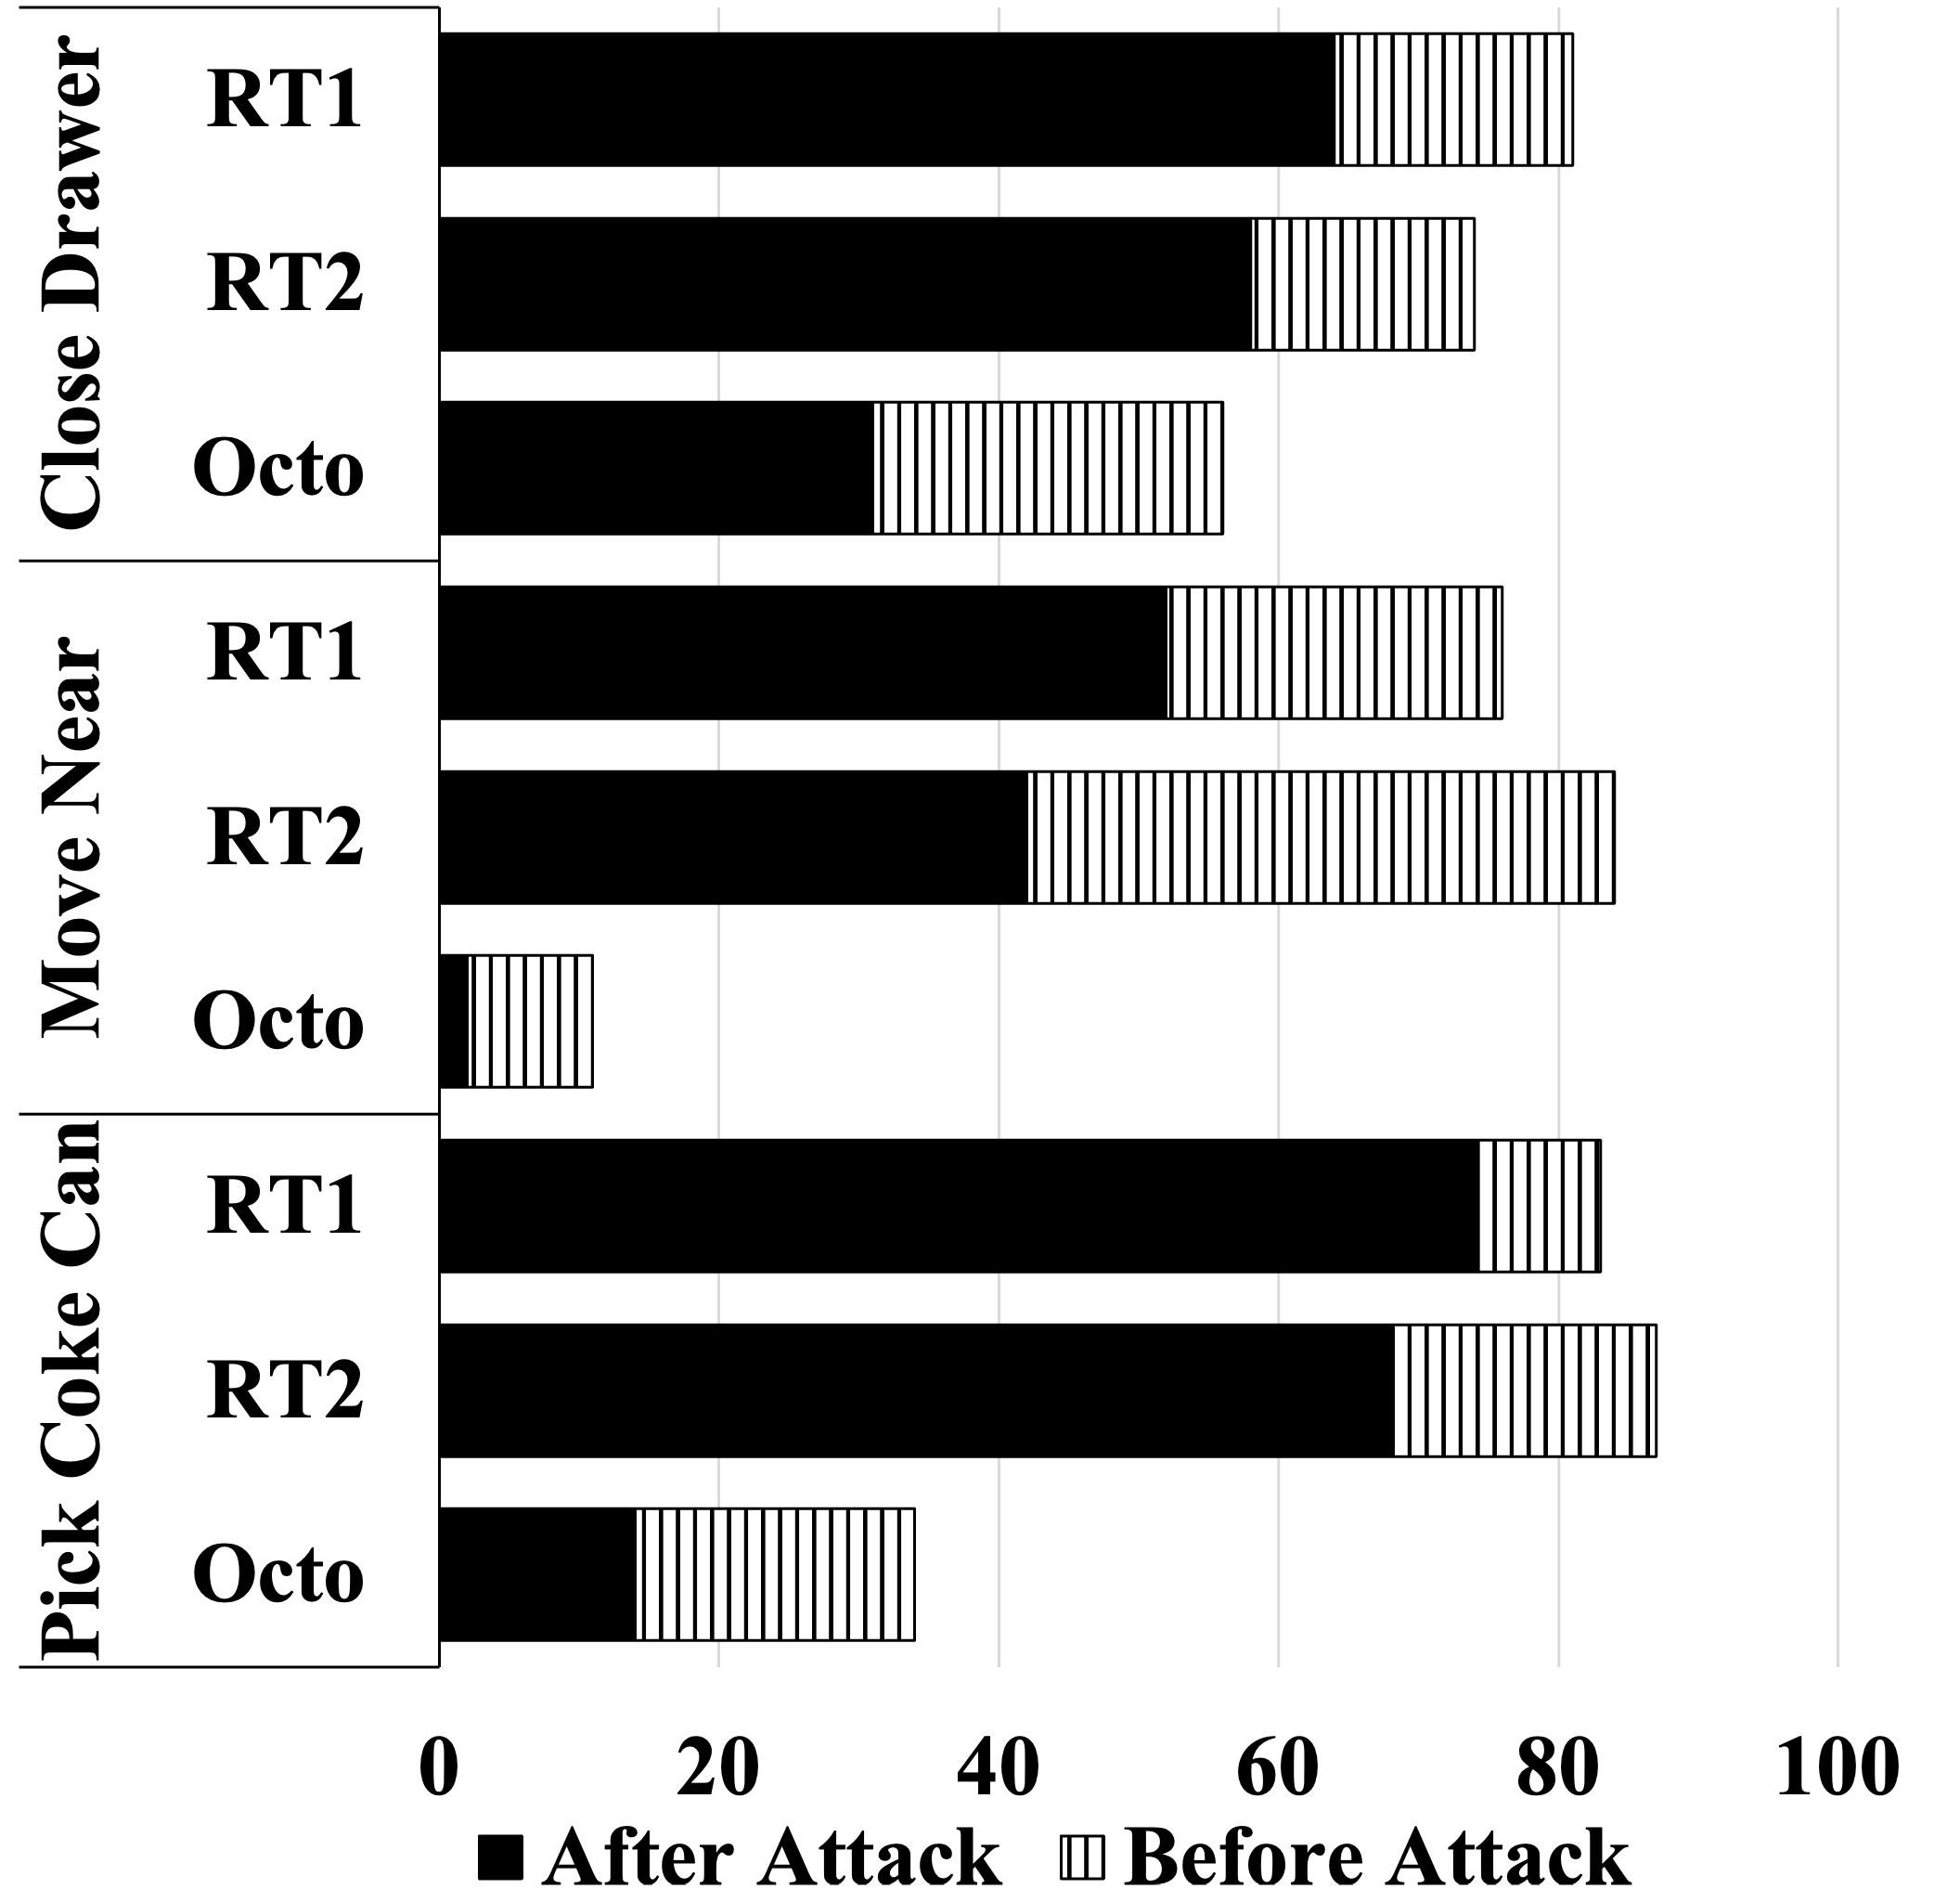
\includegraphics[width=0.9\textwidth]{figures/results/lang_white_box.pdf}\vspace{-2ex}
\caption{Task success rate of models before and after black-box token-based language perturbations.}
  \label{fig:visual_black_box}
\end{minipage}
\vspace{-5ex}
\end{wrapfigure}
 in~\autoref{fig:visual_black_box}, where we observe that the success rate of the models drops significantly after the attack, indicating that even simple token-based perturbations can disrupt the model's performance.
These results demonstrate the potential vulnerabilities of robotic models to adversarial attacks.
In these preliminary experiments we operationalized attack success as a 30\% action-token deviation proxy. In the full evaluation protocol described below, we replace this proxy with task success rate (TSR) under attack as the primary metric and retain action deviation only as a secondary physical-consequence proxy, for which we provide empirical justification through its mapping to end-effector displacement.























\subsubsection{T1-1: White-box Attacks}

White-box attacks exploit full access to the model's architecture, parameters, and gradients.
White-box attacks provide deep insights into model vulnerabilities, enabling precise identification and mitigation of weaknesses. This understanding improves the robustness and security of models, ensuring reliable and safe performance in real-world applications.
While the literature is rich in methods for white-box attacks against various models, the closest model families to generalist robot foundation models are VLMs.
Most evasion attacks against VLM \cite{schlarmann2023adversarial, bailey2023image,gao2024adversarial,wang2024stop,tan2024wolf} typically use gradient-based approaches, \eg PGD~\cite{madry2017towards}, FGSM~\cite{goodfellow2014explaining}, and CW \cite{carlini2017towards}, to generate/optimize perturbation for adversarial samples.
Recent work has begun to move beyond static, single-frame formulations toward trajectory-level redirection and architecture-specific attacks tailored to flow-matching robot policies, which we will build on and compare against~\cite{puthumanaillam2026trajectory,tae2026drift}.
As shown in \autoref{table:attacks_models}, gradient-based attacks can be performed in both the training and inference stages. During training, such attacks manipulate the model's learning process, leading to vulnerabilities such as various poisoning attacks, including recent objective-decoupled backdoor formulations tailored to VLA policies that we will study~\cite{zhou2025badvla}. At the inference stage, they generate adversarial examples by exploiting the model's gradients to deceive the model into making incorrect predictions. 
% \textit{Targeted} attacks seek to drive the model to produce a specific result or action, whereas \textit{untargeted} attacks focus on reducing the overall accuracy of the output.
A recent study \cite{fu2023misusing} shows that seemingly harmless images with trojan-like characteristics can manipulate VLMs to call attacker-specific  third-party tools or external APIs. 
In a different study~\cite{cui2023robustness}, manipulating visual contents that are different from the VLM-specific domain is less effective in deceiving the model. 
%The authorsproposed a context-augmented image classification scheme that demonstrates a significant increase. 
Gao \textit{et al.} \cite{gao2024inducing} introduce verbose images, creating imperceptible perturbations to make VLMs generate longer output sentences. Such an attack raises energy consumption and latency, which can have serious consequences in robotics.
In a cross-modal analysis, creating and refining visual perturbations using adaptive prompts can identify numerous prompts that are effective with specific visual perturbations, resulting in high transferability of adversarial samples \cite{luo2024image}.
% Wu \textit{et al.} \cite{wu2024adversarial} leverage adversarial text sequences to direct gradient-based perturbations on a single trigger image for attacking VLMs.
\ul{In this sub-task, we will propose new attack, Action-Bin Boundary Perturbation (ABBP), and investigate the cross-modal behavior and impact of various evasion and poisoning attacks on robotics models.}

\BfPara{Proposed Attack: ABBP} We propose ABBP, a gradient-based white-box attack designed to exploit the uniform 256-bin discretization of the VLA action space. Because adjacent bins encode physically close but discretely different control signals, ABBP optimizes perturbations to drive predicted action tokens across bin boundaries in a coordinated fashion across all degrees of freedom, subject to a kinematically-consistent Jacobian constraint so the induced action remains reachable. We treat PGD~\cite{madry2017towards}, FGSM~\cite{goodfellow2014explaining}, and C\&W~\cite{carlini2017towards} as baselines rather than contributions. The claimed perturbation-budget advantage over these baselines is not assumed: our formal analysis will compare the required $L_\infty$ budget after normalizing to physical consequence, since a one-bin action shift and a language-token substitution are not directly comparable units. We frame ABBP as research to be conducted, gated by a formal go/no-go check on whether action-space discretization yields a structurally distinct vulnerability.

\subsubsection{T1-2: Gray-box Attacks}
Gray-box attacks exploit partial knowledge of the model, such as its architecture or some aspects of the training pipeline/data. Gray-box attacks provide insights into model vulnerabilities, helping identify and mitigate weaknesses with moderate/limited adversarial knowledge. Multiple evasion and privacy attacks can be conducted under the gray-box scenario (see \autoref{table:attacks_models}).
Existing gray-box attacks often use other vision/language encoders or generative models as surrogates to create adversarial examples, which are transferred to attack VLMs by matching features/embeddings of different encoders to produce adversarial semantics or conceal target noises in the features/embeddings domain for better imperceptibility.
In a study by Zhao \etal \cite{zhao2024evaluating}, pre-trained CLIP \cite{radford2019language} and BLIP \cite{li2022blip} models were used as surrogate models to align adversarial perturbation with textual/image embeddings and generate transferable adversarial examples.
A recent study\cite{wang2024transferable} showed that both modality consistency and discrepancy features can help guiding highly transferable attacks through attention-directed feature perturbation to disrupt modality-consistency features in critical attention regions.
% To assess the adversarial robustness of existing VLMs in out-of-distribution scenarios, Tu \etal \cite{tu2023many} targeted the CLIP~\cite{radford2019language} image-text mismatch to mislead VLMs to produce unrelated visual responses.
In a different work~\cite{wu2024adversarial}, CLIP~\cite{radford2019language} was used as a surrogate to generate attacks against GPT-4o, Gemimi, and Claude agents that embed smaller images within larger images to generate adversarial examples. 
% Wang \etal \cite{wang2023instructta} employ a text-to-image generative model to invert the target response into a corresponding image, using the same surrogate visual encoder as the victim VLM to extract instruction-aware features from both the adversarial image and the target image. In addition, they improve transferability by using paraphrased instructions generated from an LLM.
\ul{In this sub-task, we will explore various gray-box evasion ({\eg} prompt injection and jailbreak) and privacy ({\eg} membership and attribute inference) attacks against robotics models.} Language-modality attacks ({\eg} prompt injection and jailbreak) apply only to language-conditioned models ({\eg} RT-2, OpenVLA, and Octo) and exclude vision-only models such as ACT.

\subsubsection{T1-3: Black-box Attacks}
Black-box attacks operate without any access to the model's architecture, parameters, or gradients. These attacks rely on input-output pairs to infer vulnerabilities, making it possible to identify and exploit weaknesses despite limited information about the system. 
Given their more plausible and real-world-applicable threat assumptions and adversarial capabilities, black-box attacks are challenging and critical to understanding how models can be compromised in real-world applications. 
Although numerous studies have explored and proposed various methods for such attacks on vision models~\cite{guo2019simple,hallyburton2022security,abdukhamidov2022black, juraev2024attack,abdukhamidov2023microbial} and LLMs~\cite{li2023deepinception,yao2024fuzzllm,ding-etal-2024-wolf,wei2023jailbreak,deng2024pandora}, there is limited research on these threats to VLMs~\cite{zhang2024avibench,dong2023robust} and only nascent, isolated studies targeting robotic foundation models, such as jailbreaking and backdoor attacks~\cite{badvla,advvla}, motivating the systematic study we propose here.
The lesson learned from black-box attacks against LLMs is that even with the advanced safety alignment techniques in commercial LLMs, attackers still create sophisticated methods that bypass model defenses against harmful content. 
% The incorporation of vision models and LLMs into robotic learning is receiving more attention~\cite{rt-1,rt-2,bousmalis2023robocat}, which makes it crucial to study whether inherited vulnerabilities can impact the end-to-end robotic model.
% Tan \textit{et al.} \cite{tan2024wolf} explore the indirect propagation of malicious content by subtly influencing a single 'wolf' agent to compel other 'sheep' agents in the society to produce malicious content.
% They find that this form of threat can be achieved through the indirect nature of manipulation on the input, without requiring in-depth access to the model's parameters.
A recent study~\cite{zhang2024avibench} showed that VLMs can be vulnerable to decision-based black-box visual instructions.
Moreover, Dong \etal~\cite{dong2023robust} shows that transfer-based attacks can succeed against well-defended VLMs.
Recent work has begun to construct universal, transferable adversarial patches that carry across robot policies in physical settings, which we will build on and compare against~\cite{lu2026whenrobots}.
% Wang \textit{et al.} \cite{wang2024stop} evaluate the adversarial robustness of MLLMs employing chain of thought (CoT) reasoning, finding that models using CoT generally exhibit significantly higher robustness under both answer and rationale attacks compared to models without CoT.
% Based on these findings, they introduce a novel stop-reasoning attack technique that effectively circumvents the robustness enhancements induced by CoT.
% Guo \textit{et al.} \cite{guo2024efficiently} utilize diffusion models to generate natural, unrestricted adversarial examples.
% They employ Adaptive Ensemble Gradient Estimation to ensure the adversarial examples produced contain natural adversarial semantics, thus enhancing their transferability.
% Furthermore, they use the GradCAM-guided Mask method to disperse adversarial semantics throughout the image, rather than concentrating them in a specific area, thereby improving the quality of the adversarial examples.
% Dong \textit{et al.} \cite{dong2023robust} investigate the adversarial robustness of Google's Bard as a representative of VLMs through transfer-based attacks, demonstrating that these adversarial images are highly transferable and effective at deceiving other VLMs.
% Additionally, they identify two of Bard’s defense mechanisms—face detection and toxicity detection in images—and successfully target these features in their attacks.
\ul{In this sub-task, we will explore various black-box evasion and privacy ({\eg} data reconstruction and prompt stealing) attacks against robotic models.} Language-based attacks such as prompt stealing apply only to language-conditioned models and exclude vision-only models such as ACT.

\BfPara{Proposed Attack: Temporal Trajectory Drift Attack (TTDA)} We propose TTDA, a trajectory-level gray- and black-box attack targeting the multi-step action chunk predicted by chunking policies such as Octo~\cite{team2024octo}. TTDA crafts slowly-accumulating perturbations so each individual step satisfies per-step kinematic limits and evades naive per-step anomaly checks, while the cumulative trajectory drifts toward a task-failing or workspace-violating end configuration. This attack surface is structurally absent in single-output VLMs. We will formalize sufficient conditions for such drift and characterize how chunk length affects feasibility. We will extend TTDA to flow-matching policies ({\eg} pi-0~\cite{black2024pi_0}), where the denoising trajectory provides an analogous sequence structure, as a scale-up objective in Years~3 and~4 contingent on model availability.

\subsubsection{T1-4: Defense Strategies}



 Several existing defenses (shown in~\autoref{tab:defense}) designed originally for VLMs will be examined against robotic models.
These defenses can be applied in the inference and training stages of the model development.
Inference-based defenses include anonymous detection~\cite{zhang2023mutation,gou2024eyes,pi2024mllm} and prompt engineering~\cite{wu2023jailbreaking,wang2024adashield,chen2023can} methods.% that design and optimize the prompt to enhance the defense mechanism of the model. 
JailGuard \cite{zhang2023mutation} and ECSO \cite{gou2024eyes} are designed to identify multimodal jailbreaking attacks during inference.
MLLM-Protector~\cite{pi2024mllm} proposes an inference-time detection of harmful inputs and correct (detoxify) the output responses. InferAligner~\cite{wang2024inferaligner} proposes an inference time safety alignment method for VLM. 
Alignment methods align model behaviors with expected values and intentions. The main techniques are Instruction Tuning and Reinforcement Learning from Human Feedback.
Regarding training-time VLM defenses, most work \cite{chen2023dress,zhang2023adversarial,li2024one} constructs robust natural language feedback or robust text prompts in VLM to defend against potential attacks, while \cite{li2024red,yang2024robust} proposes to train robust VLM by further fine-tuning or contrastive learning.
Recent work has begun to develop VLA-specific defenses, including structure-aware robust fine-tuning, randomized smoothing for certified robustness, and backdoor token reconstruction, which we will build on and compare against~\cite{zhang2026structure,seferis2025randomized,li2026whenattention}.
{\ul{In this sub-task, we will develop and explore the effect of various defenses against attacks on robotic models.}}
% {\vspace{-1ex}}


\BfPara{Action-Space Anomaly Detection} Beyond porting inference- and training-time VLM defenses, we propose 
a robotics-specific defense unavailable to general VLMs: an action-space anomaly detector operating on predicted actions rather than inputs. The detector flags out-of-distribution and kinematically-implausible actions, such as predictions violating the reachable workspace, joint limits, or defined safety zones, independent of the input modality under attack. Because the detector inspects the action output directly, this defense complements input-side defenses and remains effective when the compromised modality is unknown. We will characterize the detection rate and false-positive trade-off across embodiments and attack types.


\BfPara{Proposed Defenses: TACD and AGAT} We instantiate the action-space defense as the Temporal Action Consistency Detector (TACD), which raises detection from the per-step level to the sequence level to catch TTDA-style drift that per-step kinematic checks miss by construction. TACD uses a single multi-task trajectory-forecasting model conditioned on a task embedding, trained jointly on the benign demonstrations of all tasks to avoid per-task model proliferation, with a per-task threshold calibrated on held-out benign episodes. We complement detection with Action-Grounded Adversarial Fine-Tuning (AGAT), which augments fine-tuning with kinematically-constrained ABBP-style perturbations. To remain compute-feasible on the available hardware, AGAT is implemented with LoRA rank-16 adaptation (roughly 25M trainable parameters) rather than full-model backpropagation. We will evaluate TACD and AGAT against at least three baseline defenses (input smoothing, VLM-ported adversarial training, and ensemble voting), reporting detection-rate versus false-positive Pareto curves per embodiment and attack type.

\subsubsection{Evaluation Plan and Deliverables}
\begin{wraptable}{r}{0.36\textwidth}{\vspace{-3ex}}
\centering
\caption{(\textbf{T})raining \& (\textbf{I})nference defenses.}\vspace{-2ex}
\label{tab:defense}
\resizebox{\linewidth}{!}{%
\begin{tabular}{l}
\toprule
\cite{zhang2023mutation}  ~\textbf{I}$\rightarrow$  Anonymous detection \\ 
\cite{gou2024eyes}   ~\textbf{I}$\rightarrow$   Anonymous detection \\ 
\cite{pi2024mllm} ~\textbf{I}$\rightarrow$   Anonymous detection \\ 
\cite{wu2023jailbreaking}   ~\textbf{I}$\rightarrow$   Prompt engineering \\
\cite{wang2024adashield}   ~\textbf{I}$\rightarrow$   Prompt engineering \\ 
\cite{chen2023can}   ~\textbf{I}$\rightarrow$   Prompt engineering \\
\cite{wang2024inferaligner}   ~\textbf{I}$\rightarrow$   Alignment process \\
\cite{zhang2023adversarial}  ~\textbf{T}$\rightarrow$  Robust  feedback/prompt \\
\cite{chen2023dress}  ~\textbf{T}$\rightarrow$  Robust feedback/prompt \\
\cite{li2024one}  ~\textbf{T}$\rightarrow$  Robust  feedback/prompt \\
\cite{yang2024robust}  ~\textbf{T}$\rightarrow$  Fine-tuning/Contrastive learning \\
\cite{li2024red}  ~\textbf{T}$\rightarrow$  Fine-tuning/Contrastive learning \\
 \bottomrule
\end{tabular}
}\vspace{-2ex}
\end{wraptable}
We will benchmark various attacks (\autoref{table:attacks_models}) and defenses (\autoref{tab:defense}) against state-of-the-art robotic models using comprehensive datasets. Our primary metric is task success rate (TSR) under attack, a binary task-completion judgment using the two-point scoring system of our preliminary experiments. We retain the 30\% action-token deviation as a secondary physical-consequence proxy, alongside Attack Success Rate, \textit{Contain} \cite{lu2024test} (presence of attacker-specific action tokens), \textit{Exactmatch} \cite{luo2024image,lu2024test} (perfect match with attacker-specific tokens), transferability, and perturbation imperceptibility. 
To further ground these token-level metrics in physical consequences, we report maximum end-effector action displacement and the rate of safety-zone and force-threshold violations. We evaluate our proposed defenses against at least three baseline defenses, and we construct a full model~$\times$~model~$\times$~attack transferability matrix across the model families and embodiments in our scope. We report all metrics as mean~$\pm$~std over at least ten runs with multiple seeds, and assess significance with Welch's $t$-test.
We will align this protocol with recent physically-grounded evaluation practice for robot policies~\cite{sun2026maniparena}.
Deliverables include: \cib{1} a comprehensive framework of attack vectors (and defenses) specific to robotic models
with target modalities, tasks, and embodiments, \cib{2} open-source implementation includes datasets, developed attacks, defenses, and evaluations, and \cib{3} academic publications/reports/labs on findings and methodologies.




\subsection{T2: Modality-inherited Vulnerabilities and Impact on Multimodal Robots}
This task aims to examine the security and defense strategies derived from the targeting of one or more modalities used by robots. 
Although much progress has been made in designing adversarial attacks in individual modalities (\eg vision or language), the interaction between modalities remains less explored. Existing attackers, even with multimodal systems, generally treat the perturbations of different modalities separately and design them independently. 
However, this results in less interactive relations between the perturbed multimodal inputs and can be easily recognized by security alignment methods (\ie methods
to align the model behavior with expected values and intentions). 
In addition, along with visual and textual instructions, other modalities can be incorporated in the training of generalist robots. Some of these modalities can be sensory information, tabular environment data, or supplementary interpretation maps (\ie maps that indicate the region of importance in recent outputs). 

\subsubsection{Multimodal Adversarial Attacks}
To date, emerging foundation models in robotics focus mainly on visual and textual instruction. With the current trend of democratization of data and models, we expect and plan to explore more modalities as they emerge as common information used by robots.
We note that incorporating additional modalities into the system provides attackers with more physical avenues to launch attacks.
\ul{Our aim is to explore novel ways to reveal vulnerabilities by crafting ``\textit{tightly-multimodal}'' adversarial examples that simultaneously perturb visual and textual input with strong connections.} 
We will target the vision-language coupling mechanism specific to each model, namely FiLM in RT-1~\cite{rt-1}, a projection MLP in OpenVLA~\cite{kim2024openvla}, and cross-attention in Octo~\cite{team2024octo}, and formulate a model-specific co-perturbation objective at each mechanism so the visual and textual perturbations co-reinforce at the grounding layer. To test coupling on a further language-conditioned policy, we include OpenVLA-OFT or a language-conditioned Octo variant, and we exclude vision-only policies such as ACT from this multimodal scope. We present T2 as a scale-up track in Years~3 and~4 that builds on the attack baselines established in T1.
This includes studying the interactions and dependencies between modalities to create more effective cross-modal attacks that can evade current defenses. For example, Multi-key strategies~\cite{walmer2022dual} could be used to improve the connections between multimodal perturbations and co-control the attack.
Multimodal prompt injection attacks simultaneously alter both textual and visual modalities, injecting adversarial semantics into multiple modalities to enhance the possibility of overcoming alignment methods.
Recent studies \cite{qi2024visual,shayegani2023jailbreak} show that adversarial perturbations of visual and textual modalities can jointly succeed in creating malicious injections.
Recent work has begun to explore physical attention-hijacking and patch attacks that target the vision-language grounding of robot policies, which we will build on and compare against~\cite{zhang2026structure,yin2026vlaguard}.
By understanding and leveraging these interactions, we aim to develop more robust defense mechanisms that can protect against sophisticated multimodal adversarial attacks. We will also assess robustness techniques such as CleanCLIP~\cite{bansal2023cleanclip}, which retrains multimodal representations to reduce cross-modal misalignment, as a complementary defense against these attacks.
%Besides, Chen \textit{et al.} \cite{chen2023can} proposes a multimodal benchmark designed to protect specific categories of personal information in a simulated scenario. In their work, they construct textual and visual prompt injection attacks through adversarial prefixes and by rendering misinformed text onto the image, thereby inducing the model to disclose protected personal information.
\ul{In this task, variations of attacks by}~{\cite{qi2024visual,walmer2022dual}} \ul{will be implemented against robotic models.}



\subsubsection{Evaluation Plan and Deliverables}

We will benchmark various multimodal attacks, measuring their effectiveness across multiple robot embodiments and tasks. As in T1, our primary metric is task success rate (TSR) under attack, with the 30\% action-token deviation retained as a secondary proxy.
In addition to attack evaluation metrics, such as Attack Success Rate, 
\textit{Contain} \cite{lu2024test}, \textit{Exactmatch} \cite{luo2024image,lu2024test}, transferability, and imperceptibility, we will use cross-modal benign-adversarial shifting to evaluate the impact of different modality in achieving adversarial objective.
For example, assess whether the attack can succeed or change behavior when an input to a successful multimodal attack (\ie $\mathcal{M}(\mathcal{P}(\bm{x},\bm{t}_{in}))\rightarrow\bm{a}_{out}'$) is mutated, \eg $\{\mathcal{P}(\bm{x},\bm{t}_{in})\} \rightarrow\{\mathcal{P}(\bm{x}),\bm{t}_{in}\}$ or $\{\bm{x},\mathcal{P}(\bm{t}_{in})\}$.
The mutation process can be adjusted to alter the extent of shifts required to facilitate behavior change.
As in T1, we also report maximum end-effector action displacement and safety-zone and force-threshold violation rate, each as mean~$\pm$~std over at least ten runs with significance assessed by Welch's $t$-test, and we contribute the multimodal attacks to the full cross-model transferability matrix.
We will align this protocol with recent physically-grounded evaluation practice for robot policies~\cite{sun2026maniparena}.
Deliverables include: \cib{1} a comprehensive framework for multimodal attacks/defenses against robotic foundation models, analyzing how vulnerabilities propagate across modalities, \cib{2} open-source implementations of developed multimodal attacks, defenses, and benchmarks, and \cib{3} academic publications/reports/labs on findings and methodologies.

 


\subsection{T3: Benchmarks Toward Safe and Trustworthy Robotic Models}
This task aims to examine the safety and interpretability of robotic foundation models, develop methods to improve the robustness, safety, and interpretability of the models.
The importance of trustworthiness in robotic models cannot be overstated, particularly as large foundation models in robotics continue to emerge and possibly integrate in multiple downstream tasks within various sectors. 
Ensuring the safety of these robotic systems is paramount, as any malfunction or unexpected behavior can cause significant harm or damage in environments where robots operate alongside humans. 
Transparency is another challenge for these models and systems.
Generally, transparency (\ie explainability or interpretability) poses a major challenge in large multimodal models, given that intricate models and the combination of various input types can produce actions that are not easily understood.
% This lack of transparency can obscure potential biases embedded within algorithms/data, leading to unfair or discriminatory outcomes. 
Solving these challenges requires rigorous testing benchmarks and protocols to ensure that robotic models perform reliably, safely, and uphold ethical integrity.



\subsubsection{T3-1: Safety in Robotic Models}
Ensuring safety has been a crucial aspect of robotics since the introduction of the earliest industrial robots.
Safety, defined as the condition of being protected from or unlikely to cause danger, risk, or injury, is a critical issue in Industrial Robotics, where more than 1.5 million industrial robots operate in factories worldwide.
Although there are high standards of operational safety of robotics, such as ISO 13482:2014 personal care robots, ISO 10218-1 and ISO 10218-2 for industrial robots, and ISO/TS 15066 for collaborative robots, safety in foundation robotic models should address possible harm or bias in output given certain inputs (benign or adversarial).
In relation to such safety aspects, there have been no previous works that addressed such issues, except physical safety~\cite{FoschVillaronga2015CreationOA,RePEc:eps:cepswp:26204,10.3389/frobt.2022.1002226}.
A study by~\cite{fosch21} explores the interaction between robots, cybersecurity, and safety from a European legal perspective, illustrating cybersecurity challenges and their subsequent safety implications with the concrete example of care robots.
Another study by~\cite{tadokoro19} provides an overview of the ImPACT Tough Robotics Challenge and Strategy for Disruptive Innovation in Safety and Security (ImPACT-TRC), a project by the Japan Cabinet Office focusing on robotic technologies for disaster response, recovery, and preparedness.
To ensure the safety of the robot model, an effective and innovative validation process is crucial. This is difficult due to the restricted number of validation scenarios which may fail to reflect real-world intricacies, along with the significant computational expense of identifying infrequent failures.
Several prior studies have established standardized push-recovery testbeds by imposing consistent external perturbations on the legged robot under varying control strategies \cite{zhangei2023quadruped-tro, weng2023standard-legged-test, weng2023comparability}.
Recent work has begun to release dedicated VLA security benchmarks and physically-grounded evaluation suites, which we will build on and compare against~\cite{li2025attackvla,sun2026maniparena}.

\ul{To evaluate the safety measures of generalist robot models, we propose examining various defense mechanisms that enhance robustness and safety. We will develop methods similar to JailGuard~}\cite{zhang2023mutation}\ul{, ECSO~}\cite{gou2024eyes}\ul{,  MLLM-Protector~}\cite{pi2024mllm}\ul{, InferAligner~}\cite{wang2024inferaligner}\ul{ to detect/normalize safety-critical outputs during inference.}


\subsubsection{T3-2: Interpretation of Robotic Models}

Regardless of the architecture or domain, it is essential that we can interpret and explain the decisions made by the AI model.
Methods for interpretability can be categorized into gradient- and inference-based methods. 
Gradient-based methods typically leverage inter- and intra-modality interactions to provide visual explanations for the decisions, whereas inference-based methods are designed to provide explanations to specific aspects or components of the models and may be limited to particular tasks.




\BfPara{Gradient-based Interpretation Methods} 
Robotic models are mostly incorporate transformer-based components, which can use
attention maps for interpretation. 
Variants of these methods have been discussed in the literature, such as the Attention Rollout \cite{abnar2020quantifying}, which integrates layers to produce an average attention map. %The work by~\cite{voita-etal-2019-analyzing} specifically adapted the LRP method for transformers, addressing computational challenges.
A recent study \cite{DBLP:journals/corr/abs-2106-12620} proposes $\text{IA-RED}^2$, enhancing transformer efficiency with human-understandable architecture.
Other methods include AttCAT~\cite{DBLP:conf/nips/QiangPLLJZ22}, B-cos~\cite{DBLP:journals/corr/abs-2301-08669}, Vision DiffMask~\cite{DBLP:conf/cvpr/NalmpantisPGPA23}, and ICE~\cite{DBLP:conf/cvpr/ChoiJH23}.
In the VLM domain and multimodal interpretation, Relevancy Map \cite{chefer2021generic} uses self-attention and co-attention with classification tokens to produce a relevancy map, tracking interactions across modalities, and back-propagating relevancies. The approach works for unimodal and multimodal models.
VL-InterpreT \cite{aflalo2022vl} serves as a tool providing an interactive interface to examine the interactions among the modalities using a bottom-up approach. It employs four modality attention heads: language-to-vision attention, vision-to-language attention, language-to-language attention, and vision-to-vision attention, enabling the examination of interactions both within and across modalities.
Other methods include MultiViz \cite{liang2022multiviz} and gScoreCAM~\cite{chen2022gscorecam}.
 



\BfPara{Inference-based Interpretation Methods} 
Most interpretation techniques for VLMs rely on inference-based methods, which are designed to investigate specific components of the model, making them difficult to generalize. 
The Vision And Language Understanding Evaluation (VALUE) method described in \cite{cao2020behind} introduces various inference tasks aimed at understanding the impact of pre-training on learned representations.
The research indicates that pre-trained VLMs prioritize language over vision and that some attention heads are responsible for capturing interactions across modalities.
In another study~
\cite{dahlgren-lindstrom-etal-2020-probing}, three inference tasks for visual-semantic space were introduced to capture image-caption relations.
% A study by~\cite{hendricks2021probing} presents inference tasks for verb understanding using image-sentence pairs with 421 verbs from the Conceptual Captions dataset~\cite{sharma2018conceptual}. 
A study by~\cite{DBLP:conf/aaai/SalinFAF22} introduces inference tasks to understand and compare representations by VLMs from pre-trained and finetuned versions. 


%In addition, data sets are designed carefully for multimodal
%probing, trying to reduce dependency on bias while making predictions. While probing tasks are helpful and can answer meaningfully with regard to particular problems, they have to be carefully crafted for relevant results and are very specific. At times, extra models or classifiers are required for probing, making the probing tasks applicable to selected models only.


\ul{We aim to investigate both gradient- and inference-based techniques to better understand predicted robotic actions. We will develop methods to interpret the decisions made by robotic models.}
Recent work has begun to explore spatial-grounding attribution and neuro-symbolic spatial reasoning for embodied models, which we will build on for action-level interpretation~\cite{schofield2026chain,jahangard2025multimodal}.


\subsubsection{Evaluation Plan and Deliverables}
Visualization techniques, \eg heatmaps and saliency maps, will be used to interpret how the model makes decisions under both normal and adversarial conditions.
Case studies on specific instances (\ie instruction-action pairs) where the model fails or succeeds will be conducted to understand the behavior of the model.
There will be human-in-the-loop evaluations that include reviewing and interpreting the results, ensuring that the methods align with human understanding and expectations.
Deliverables include: \cib{1} benchmarks for safety and interpretability of robotic foundation models, \cib{2} open-source implementations of developed safety and interpretability methods, and \cib{3} academic publications/reports/labs on findings and methodologies.


\subsection{Work Plan, Timeline, and Team}

\BfPara{Staged Scope} We stage the program into Phase 1 (Years~1 and~2) and a Phase 2 (Years~3 and~4). Phase 1 targets open and architecturally complementary models on two embodiments (Xarm7 and the Google robot), and develops ABBP and TTDA with ported baselines together with the TACD and AGAT defenses and their baselines. 
The Phase 2 adds emerging models, multimodal analysis, certified-robustness defenses, and the full public release of VLA-SecBench. 
\autoref{fig:workplan_timeline} summarizes the schedule of the research-plan tasks under the calendar aligned to the budget period.

\begin{figure*}[t]
\centering
\resizebox{\textwidth}{!}{%
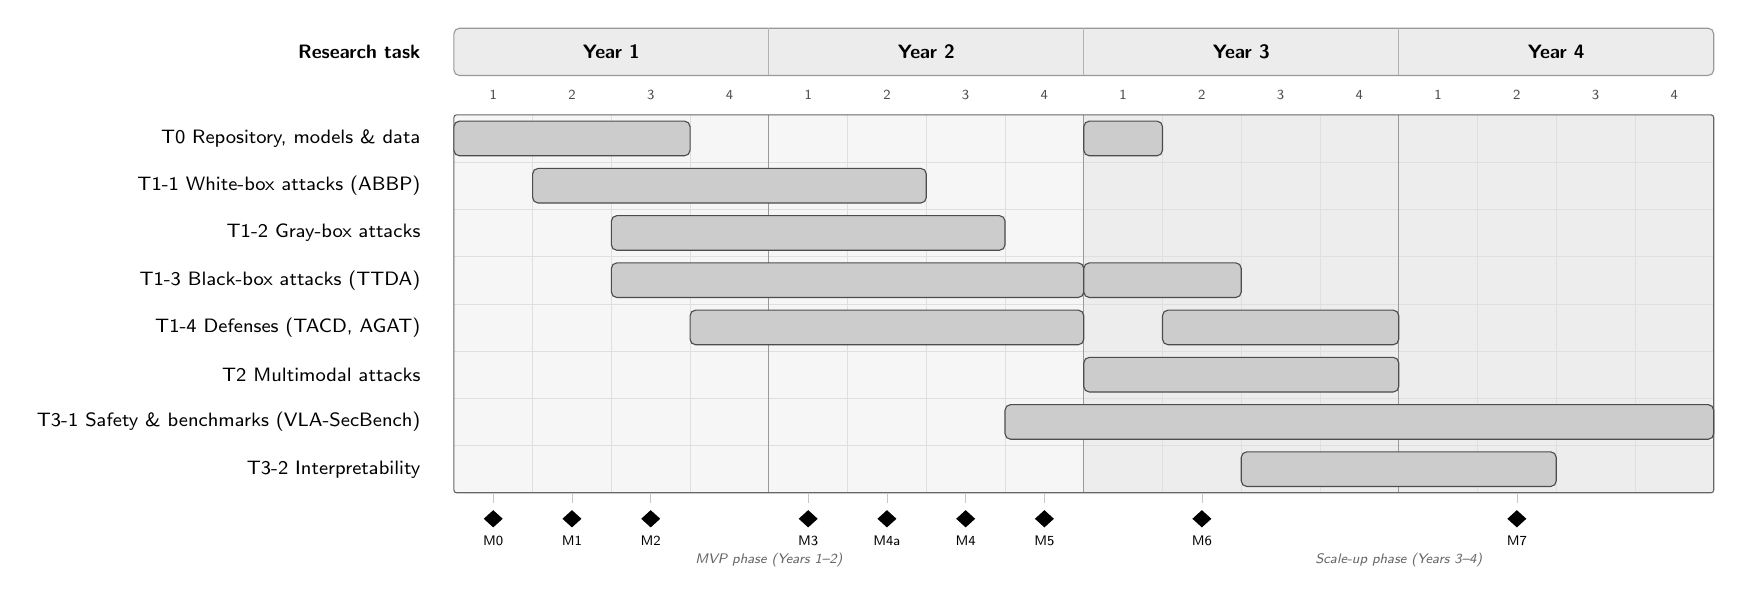
\begin{tikzpicture}[font=\scriptsize\sffamily,
  bar/.style={fill=gray!40, draw=black!70, rounded corners=2pt},
  ]
  %%% phase (MVP / Scale-up) background shading %%%
  \fill[gray!7]  (0,-3.4) rectangle (8,1.4);
  \fill[gray!14] (8,-3.4) rectangle (16,1.4);

  %%% horizontal row separators %%%
  \foreach \hy in {0.80,0.20,-0.40,-1.00,-1.60,-2.20,-2.80}
    \draw[very thin, gray!25] (0,\hy) -- (16,\hy);

  %%% vertical quarter gridlines %%%
  \foreach \gx in {1,2,3,5,6,7,9,10,11,13,14,15}
    \draw[very thin, gray!25] (\gx,-3.4) -- (\gx,1.4);
  %%% year boundary lines %%%
  \foreach \gx in {4,8,12}
    \draw[thin, black!40] (\gx,-3.4) -- (\gx,1.4);
  %%% outer chart border %%%
  \draw[black!60, rounded corners=1pt] (0,-3.4) rectangle (16,1.4);

  %%% year header band %%%
  \fill[gray!15, draw=black!40, rounded corners=2pt] (0,1.9) rectangle (16,2.5);
  \foreach \gx in {4,8,12} \draw[black!30] (\gx,1.9) -- (\gx,2.5);
  \node[font=\scriptsize\bfseries\sffamily] at (2,2.2)  {Year 1};
  \node[font=\scriptsize\bfseries\sffamily] at (6,2.2)  {Year 2};
  \node[font=\scriptsize\bfseries\sffamily] at (10,2.2) {Year 3};
  \node[font=\scriptsize\bfseries\sffamily] at (14,2.2) {Year 4};

  %%% quarter tick numbers %%%
  \foreach \g in {1,...,16} {
    \pgfmathtruncatemacro{\qn}{mod(\g-1,4)+1}
    \node[font=\tiny\sffamily, text=black!70] at (\g-0.5,1.65) {\qn};
  }

  %%% left-hand labels %%%
  \node[anchor=east, font=\scriptsize\bfseries\sffamily] at (-0.3,2.2)  {Research task};
  \node[anchor=east] at (-0.3,1.10)  {T0 Repository, models \& data};
  \node[anchor=east] at (-0.3,0.50)  {T1-1 White-box attacks (ABBP)};
  \node[anchor=east] at (-0.3,-0.10) {T1-2 Gray-box attacks};
  \node[anchor=east] at (-0.3,-0.70) {T1-3 Black-box attacks (TTDA)};
  \node[anchor=east] at (-0.3,-1.30) {T1-4 Defenses (TACD, AGAT)};
  \node[anchor=east] at (-0.3,-1.90) {T2 Multimodal attacks};
  \node[anchor=east] at (-0.3,-2.50) {T3-1 Safety \& benchmarks (VLA-SecBench)};
  \node[anchor=east] at (-0.3,-3.10) {T3-2 Interpretability};

  %%% research-task bars (active quarters) %%%
  \fill[bar] (0,0.88)   rectangle (3,1.32);   % T0
  \fill[bar] (8,0.88)   rectangle (9,1.32);   % T0 (refresh)
  \fill[bar] (1,0.28)   rectangle (6,0.72);   % T1-1
  \fill[bar] (2,-0.32)  rectangle (7,0.12);   % T1-2
  \fill[bar] (2,-0.92)  rectangle (8,-0.48);  % T1-3
  \fill[bar] (8,-0.92)  rectangle (10,-0.48); % T1-3 (extend)
  \fill[bar] (3,-1.52)  rectangle (8,-1.08);  % T1-4
  \fill[bar] (9,-1.52)  rectangle (12,-1.08); % T1-4 (certified)
  \fill[bar] (8,-2.12)  rectangle (12,-1.68); % T2
  \fill[bar] (7,-2.72)  rectangle (16,-2.28); % T3-1
  \fill[bar] (10,-3.32) rectangle (14,-2.88); % T3-2

  %%% milestone diamonds along the bottom axis %%%
  \foreach \mx/\ml in {0.5/M0, 1.5/M1, 2.5/M2, 4.5/M3, 5.5/M4a, 6.5/M4, 7.5/M5, 9.5/M6, 13.5/M7} {
    \draw[very thin, gray!45] (\mx,-3.4) -- (\mx,-3.53);
    \fill[black, draw=black] (\mx,-3.63) -- (\mx-0.11,-3.73) -- (\mx,-3.83) -- (\mx+0.11,-3.73) -- cycle;
    \node[font=\tiny\sffamily, anchor=north, inner sep=1pt] at (\mx,-3.9) {\ml};
  }

  %%% phase captions %%%
  \node[font=\tiny\itshape\sffamily, text=black!60] at (4,-4.25)  {MVP phase (Years 1--2)};
  \node[font=\tiny\itshape\sffamily, text=black!60] at (12,-4.25) {Scale-up phase (Years 3--4)};
\end{tikzpicture}%
}
\caption{Gantt-style work-plan timeline. Calendar aligned to the anticipated award start (May~2027): Year~1 = May~2027--Apr~2028, \ldots, Year~4 = May~2030--Apr~2031; quarters Q1~(May--Jul), Q2~(Aug--Oct), Q3~(Nov--Jan), Q4~(Feb--Apr). Bars indicate active quarters; diamonds mark milestones (M0--M7). {\footnotesize\textbf{Milestones:} \textbf{M0} compute/NSF ACCESS allocation secured; \textbf{M1} ABBP formal specification; \textbf{M2} MVP model zoo operational; \textbf{M3} ABBP vs.\ PGD comparison; \textbf{M4a} preliminary TACD false-positive check; \textbf{M4} formal TACD detection gate; \textbf{M5} VLA-SecBench v0.5 \& pi-0 availability; \textbf{M6} multimodal coupling benefit shown; \textbf{M7} VLA-SecBench v1.0 release.}}
\label{fig:workplan_timeline}
\end{figure*}




% \subsection{Task Implementation and Timeline}

% \begin{figure*}[h]
%   \centering\vspace{-2ex}
%   \includegraphics[width=0.63\textwidth]{figures/grant1_1.pdf}\vspace{-2ex}
%   \caption{Proposed work plan and timeline.}
%   \label{fig:timeline}
% \end{figure*}
